\chapter[LANDASAN TEORI]{\\ LANDASAN TEORI}

\section{Tinjauan Pustaka}
\subsection{Studi Kasus Library JavaScript dan Visualisasi Data}
Guna melakukan perbandingan terhadap Chart.js, Highcharts, dan D3.js, penulis meninjau sumber-sumber yang berkaitan dengan penggunaan library-library tersebut dalam memvisualisasikan data perangkat IoT berukuran besar, beberapa diantaranya adalah studi yang dilakukan oleh Vučetić [11] Manna dan Banerjee [12], Toppany et.al [13], dan Rothenhausler [14].

Pada jurnalnya yang berjudul “Open Data Visualization by Using Javascript Libraries”, Vučetić [11] melakukan penelitian mengenai visualisasi data open source menggunakan library JavaScript, dengan fokus pada data dari pemerintahan yang dapat diakses secara bebas. Setelah melakukan perbandingan terhadap beberapa library visualisasi, Vučetić memilih Highcharts sebagai library untuk menampilkan data grafik statistik yang memungkinkan pengguna melihat jumlah perpustakaan berdasarkan distrik. Untuk pembuatan peta Interaktif yang menampilkan lokasi perpustakaan di berbagai distrik, Vučetić menggunakan Leaflet.js. 

Manna dan Banerjee [12] mengimplementasikan Highcharts dalam pengembangan visualisasi perangkat IoT. Dalam implementasinya, Highcharts digunakan sebagai alat visualisasi data real-time pada user interface (UI) berbasis web. Highcharts dipilih karena kemampuannya menampilkan data sensor secara interaktif, termasuk suhu ruangan, tingkat cahaya, dan aktivitas akses pintu berbasis RFID. Dalam sistem ini, Highcharts diintegrasikan dengan HTML dan JavaScript untuk menampilkan grafik dinamis yang diperbarui secara otomatis tanpa perlu refresh halaman. Grafik yang digunakan mencakup grafik perbandingan cahaya dan waktu, grafik perbandingan suhu dan waktu, dan log akses RFID, yang dihasilkan dari data yang dikirimkan oleh sensor melalui MQTT broker di AWS. Dengan Highcharts, pengguna dapat memantau kondisi secara real-time, melihat detail titik data dengan fitur hover dan zoom, serta memahami tren perubahan lingkungan dengan lebih mudah.

Pada sebuah penelitian dengan judul “Integrasi Framework Bootstrap dan Chart.js untuk Visualisasi Data Sensor pada Sistem Hidroponik Berbasis Internet of Things (IoT)” yang dilakukan oleh Toppany et.al [13], peneliti mengembangkan sistem visualisasi data sensor berbasis Internet of Things (IoT) yang dapat diakses melalui website. Pengujian dan evaluasi sistem ini mencakup responsivitas website, kecepatan pemrosesan data, serta kestabilan sistem dalam menangani banyak pengguna. Hasilnya, website yang dikembangkan dapat memuat halaman dalam 2 detik dan menangani user request dengan latensi 354 ms. Sistem berhasil menampilkan data suhu, pH, dan TDS air secara real-time dalam bentuk grafik. Pengujian dengan 500 user dalam satu menit. Hal ini menunjukkan bahwa website dapat menangani beban tanpa mengalami crash. Delay dalam pengiriman data dari ESP-32 ke website rata-rata 12 menit 1 detik, dikarenakan sistem dirancang untuk melakukan sampling data secara berkala guna mencegah overload database. 

Dalam penggunaan D3.js, Rothenhausler [14] melakukan studi untuk menganalisis performa D3.js dalam memvisualisasikan data pengungsi Ukraina akibat konflik bersenjata. Dalam penelitian ini, D3.js dijelaskan sebagai library yang memberikan kontrol penuh terhadap manipulasi elemen dalam Document Object Model (DOM) yang akan memudahkan pengembang untuk membuat chart yang fleksibel. Penelitian ini menguji performa D3.js dalam menangani jumlah elemen yang besar dalam sebuah diagram. Hasil dari penelitian ini menunjukkan, animasi pada D3.js bekerja dengan baik hingga batas tertentu. D3 melakukan manipulasi langsung pada DOM, sehingga dapat menyebabkan lag jika terlalu banyak elemen yang diperbarui secara bersamaan. Berdasarkan hasil pengujian terhadap kemampuan render, pada dataset hingga 1200 elemen, D3 bisa berjalan lancar, tetapi di atas itu, diperlukan optimasi tambahan atau beralih ke teknologi berbasis Canvas/WebGL untuk performa yang lebih baik. 

Dalam melakukan pengambilan data, penulis perlu mempertimbangkan data yang akan digunakan agar sesuai dengan data lapangan. Dalam hal ini, penulis merujuk pada jurnal penelitian “Sistem Pemantauan Lingkungan Menggunakan Sensor BME280 Berbasis Internet of Things” [15]. Penelitian ini mengembangkan sistem pemantauan lingkungan berbasis Internet of Things (IoT) dengan menggunakan sensor BME280 yang mampu mengukur parameter suhu, kelembaban, tekanan udara, dan ketinggian. Sistem ini menggunakan NodeMCU ESP8266 sebagai mikrokontroler yang bertugas mengumpulkan data sensor dan mengirimkannya ke platform ThingSpeak untuk penyimpanan dan visualisasi. Proses pengambilan data dilakukan secara berkala untuk memastikan keakuratan hasil pemantauan. Akuisisi data dari sensor BME280 dilakukan setiap 10 detik, dengan 10 sampel digunakan untuk kalkulasi Median Filter sebelum data dikirim ke server. Setelah proses filtering, data disimpan di platform ThingSpeak setiap ±45 detik, karena adanya batasan pembaruan minimum per 15 detik di platform tersebut. 

Untuk mnentukan batas jumlah data maksimal pada halaman website, penulis menggunakan rujukan jurnal dari Melo et al. dalam judul “A Low-Cost IoT System for Real-Time Monitoring of Climatic Variables and Photovoltaic Generation for Smart Grid Application” [16]. Jurnal ini membahas pengembangan dashboard monitoring cuaca secara real-time melalui MQTT dan membuat visualisasi dengan Chart.js. Dalam pengembangannya, dashboard ini hanya menampilkan 1440 titik data untuk menjaga kelancaran rendering, kemudian mengganti data terlama saat ada titik baru. 

\begin{longtable}{|p{\dimexpr.35\linewidth-2\tabcolsep-1.25\arrayrulewidth}|
		p{\dimexpr.20\linewidth-2\tabcolsep-1.25\arrayrulewidth}|
		p{\dimexpr.45\linewidth-2\tabcolsep-1.25\arrayrulewidth}|}
	\caption{Perbandingan penelitian} \label{t_risetPemodelan} \\
	\hline
	\textbf{Judul} & \textbf{\textit{Library/ Tools }} & \textbf{Studi Kasus} \\ \hline
	\endfirsthead
	
	\multicolumn{3}{c}{} \\ \hline
	\textbf{Judul} & \textbf{\textit{Library/ Tools }} & \textbf{Studi Kasus} \\ \hline
	\endhead
	
	\hline \multicolumn{3}{r}{ } \\ 
	\endfoot
	
	\hline
	\endlastfoot
	
	\textit{“Open Data Visualization by Using Javascript Libraries”} [11] &Leaflet.js, HighChart.js, Chart.js, dan D3.js. & Library Highcharts digunakan untuk memvisualisasikan data grafik yang menampilkan jumlah perpustakaan berdasarkan distrik. \\ \hline
	\textit{“Experimental Study on MQTT Protocol Based Home Automation System with Enhancement”} [12] & Highcharts & Highcharts digunakan dalam UI berbasis web untuk menampilkan data sensor secara real-time seperti suhu ruangan, tingkat cahaya, dan aktivitas akses pintu berbasis RFID, dan menyediakan grafik interaktif yang memungkinkan pengguna melihat tren data dari waktu ke waktu, serta mendukung pemantauan jarak jauh. grafik dapat diperbarui secara real-time dan Highcharts mampu menangani data dari berbagai sensor dengan latensi rendah.\\ \hline
	\textit{“Integrasi Framework Bootstrap dan Chart.js untuk Visualisasi Data Sensor pada Sistem Hidroponik Berbasis Internet of Things (IoT)”} [13] & Chart.js & 
	\begin{itemize}
		\item[-] Memuat halaman dalam 2 detik dan menangani user request dengan latensi 354 ms. 
		\item[-]  Pengujian dengan 500 pengguna dalam 1 menit menunjukkan bahwa situs web dapat menangani beban tanpa mengalami crash.
		\item[-] Delay dalam pengiriman data dari ESP-32 ke website rata-rata 12 menit 1 detik, dikarenakan sistem dirancang untuk melakukan sampling data secara berkala guna mencegah overload database.
	\end{itemize} \\ \hline
	\textit{“d3.js and its potential in data visualization Creating a diagram showcase using Ukrainian refugee data”} [13] & D3 & 
	D3 mampu menangani hingga 1200-1300 elemen animasi secara smooth, tetapi performa mengalami penurunan karena kompleksitas visualisasi dan spesifikasi perangkat yang digunakan. \\ \hline
	\textit{“Sistem Pemantauan Lingkungan Menggunakan Sensor BME280 Berbasis Internet of Things”} [13] & Sensor BME280 & 
	Durasi pengambilan data kurang lebih 45 detik. Hal tersebut meliputi interval antar data (10 detik) dan proses pengiriman data ke ThinkSpeak termasuk proses median filter serta perhitungan latensi(20-35 detik). \\ \hline
	\textit{“A Low-Cost IoT System for Real-Time Monitoring of Climatic Variables and Photovoltaic Generation for Smart Grid Application”} [13] & Chart.js & 
	 Jurnal ini memvisualisasikan data real-time dengan Chart.js dan membatasi data yang ditampilkan pada Chart.js sebanyak 1440 data untuk mengefisienkan performa rendering. \\ \hline
\end{longtable}

Berdasarkan kajian pustaka yang telah dilakukan, Chart.js, D3.js, dan Highcharts dapat diimplementasikan sebagai chart untuk menampilkan data-data IoT. Tiap-tiap library ini memiliki kelebihan dan kekurangannya masing-masing. Oleh karena itu, library-library tersebut akan diujikan dengan data dummy yang telah disamakan formatnya dengan data IoT asli yang merujuk pada jurnal-jurnal yang telah disebutkan sebagai referensi untuk menguji kemampuannya dalam menampilkan data dalam jumlah tertentu. 

\subsection{Studi Analisis Perbandingan}
Untuk melakukan penelitian ini, penulis meninjau berbagai sumber pustaka akademik yang membahas topik serupa yaitu perbandingan antara library visualisasi JavaScript, sebagai landasan sekaligus bahan perbandingan. Studi-studi ini melakukan penelitian dengan metode dan berbagai library JavaScript selain ChartJS, Highcharts, dan D3.js. 

Danielyan [18] melakukan penelitian untuk meninjau perbandingan library visualisasi JavaScript dalam judul "Analysis of Data Visualization Tools and Approaches". Studi ini menganalisis berbagai tools visualisasi data berdasarkan aspek biaya, kemudahan penggunaan, kemampuan, serta dokumentasi dan dukungan. Library yang diujikan pada penelitian ini adalah D3.js, Chart.js, Chartist.js, FusionCharts, dan Google Charts. Hasilnya, pada  parameter popularitas,  D3.js menjadi library paling populer dengan lebih dari 80.000 GitHub stars. Dari parameter kemudahan penggunaan, Chart.js, Chartist.js, dan Google Charts cenderung lebih mudah karena berbasis chart object constructor, dan D3.js menjadi library yang paling customizable namun membutuhkan lebih banyak kode. Dari parameter jenis chart, FusionCharts menyediakan lebih dari 95 jenis chart bawaan, termasuk grafik geospasial. Google Charts mendukung lebih dari 25 tipe chart akan tetapi membutuhkan koneksi internet dalam implementasinya. 

Gokhale dan Mahajan [19] dalam penelitiannya yang berjudul Comparative “Study of Data Visualization Tools” membandingkan berbagai alat visualisasi data berdasarkan beberapa aspek utama, yaitu ketersediaan open-source, kebutuhan pemrograman, bahasa pemrograman yang digunakan, serta jenis output grafis yang dihasilkan. Dari segi ketersediaan, beberapa library bersifat open-source dan dapat digunakan secara gratis, seperti D3.js, Chart.js, Leaflet, Dygraphs, Google Charts, dan Timeline.js. Sementara itu, terdapat pula library yang bersifat komersial dan memerlukan lisensi, seperti Microsoft Excel, Highcharts, dan FusionCharts, yang umumnya menawarkan fitur lebih lengkap bagi pengguna. Dalam hal kebutuhan pemrograman, Microsoft Excel dan Timeline.js, dapat digunakan tanpa pemrograman, sehingga lebih mudah diakses oleh pengguna yang tidak memiliki latar belakang teknis. Sebaliknya, library seperti D3.js, Chart.js, Highcharts, Leaflet, Dygraphs, FusionCharts, dan Google Charts memerlukan pemahaman bahasa pemrograman, khususnya JavaScript. Sementara itu, Microsoft Excel menggunakan Visual Basic for Applications (VBA) untuk kebutuhan analisis data yang lebih kompleks. Dari segi jenis output grafis yang dihasilkan, Microsoft Excel, D3.js, Chart.js, Highcharts, FusionCharts, dan Google Charts banyak digunakan untuk menghasilkan berbagai jenis grafik, seperti bar chart, line chart, dan pie chart sementara D3.js, Highcharts, Google Charts, dan Dygraphs, juga dapat digunakan untuk memvisualisasikan bar chart, line chart, dan pie chart dengan fitur yang lebih interaktif. Untuk visualisasi berbasis peta, Leaflet merupakan pilihan utama, sedangkan Timeline.js lebih cocok untuk menampilkan data dalam bentuk time-series yang interaktif.

Dalam penelitiannya yang berjudul “Scalability of JavaScript Libraries for Data Visualization”, Persson [4] melakukan analisis dengan tujuan mengetahui apakah ukuran dataset dan/atau jenis grafik mempengaruhi waktu render pada library JavaScript yang dibandingkan dan apakah tipe chart mempengaruhi performa rendering. Hasilnya, ukuran dataset mempengaruhi waktu render pada semua jenis chart. Hasil ANOVA-test menunjukkan p-value sebesar 0,61 dengan confidence level 95\% yang berarti tidak ada perbedaan yang signifikan dalam waktu render antara grafik garis dan diagram batang ketika dataset terdiri dari 100 titik data. Hasilnya serupa untuk set data 5 ribu titik dengan nilai p-value 0,54 dan confidence level 95\% dan dengan demikian tidak ada perbedaan yang signifikan perbedaan waktu render antara diagram garis dan batang ketika dataset terdiri dari 5 ribu titik.

Bennba juga turut melakukan penelitian mengenai library Javascript untuk visualisasi dalam judul tesisnya “Comparison of D3.js and Chart.js as Visualization Tools” [20]. Dalam tesisnya, Bennba melakukan perbandingan terhadap Chart.JS dan D3.js untuk melakukan uji performa pada waktu eksekusi, load time, dan penggunaan memori. Uji performa dilakukan dengan memvisualiasikan data menggunakan line chart dan untuk membuat grafik garis dengan dataset berukuran 10, 100, 1.000, 10.000, 100.000, dan 1.000.000 data. Hasilnya, D3.js lebih cepat dibandingkan Chart.js dalam hal waktu eksekusi, terutama pada dataset besar. Sementara itu, Chart.js mengalami crash saat mencoba merender 1.000.000 data. Sedangkan dalam hal penggunaan memori, jika setiap titik data dirender sebagai elemen SVG individual, D3 mengalami  peningkatan konsumsi memori secara drastis.

Penelitian serupa juga dilakukan oleh Bostromm, dkk [3] dalam judul “A performance investigation into JavaScript visualization libraries with the focus on render time and memory usage”. Penelitian ini bertujuan untuk menentukan apakah ukuran dataset mempengaruhi waktu render dan penggunaan memori, baik di dalam library itu sendiri maupun di antara semua library JavaScript yang dipilih serta meneliti apakah terdapat perbedaan waktu render yang signifikan ketika terdapat peningkatan poin data. Hasilnya, ukuran dataset mempengaruhi waktu render. Semua library mengalami peningkatan waktu render seiring bertambahnya jumlah data, kecuali dalam beberapa kasus anomali, seperti ECharts yang menunjukkan waktu render lebih rendah di kategori 2 dibanding kategori 1. Selain itu, ANOVA test menunjukkan nilai p > 0.05 ketika membandingkan waktu render antara line chart dan bar chart, baik untuk dataset kecil (100 data) maupun besar (5000 data), sehingga tidak ada perbedaan signifikan antara kedua tipe chart ini. 

Perbandingan performa render dan waktu respon juga diteliti oleh Millqvist dan Bolin [21] dalam tesisnya yang berjudul “A Comparison of Performance and Scalability of Chart Generation for Javascript Data Visualization Libraries”. Studi ini membandingkan performa lima library JavaScript, yaitu Chart.js, ApexCharts, Billboard.js, ToastUI, dan Chartist dengan fokus penelitian untuk mengukur waktu respon dalam merender pie charts, bar charts, line charts, dan scatter plots. Pengujian dilakukan dengan parameter waktu respons dari setiap library dalam merender grafik, skalabilitas berdasarkan ukuran dataset (dari 100 hingga 1.000.000 data), serta normalisasi grafik. Hasil dari penelitian ini menunjukkan bahwa Chart.js dapat memproses hingga 1.000.000 data tanpa mengalami crash. Chartist memiliki performa render yang cepat tetapi gagal merender dataset besar (>100.000 data). Sedangkan ApexCharts dan Billboard mengalami kendala eksponensial seiring dengan meningkatnya waktu respon. Dari kelima library yang diujikan, Chart.js adalah pustaka paling stabil yang mampu menangani semua ukuran dataset tanpa mengalami crash. 

Kim et al [22], dalam jurnal penelitiannya yang berjudul “Beyond Alternative Text and Tables: Comparative Analysis of Visualization Tools and Accessibility Methods”, meninjau tentang penggunaan library JavaScript, termasuk Highchart dan Tableau dalam pengembangan website yang mendukung aksesibilitas dan skalabilitas. Penulis melakukan analisis terhadap 39 alat visualisasi data berbasis web, termasuk 30 library pemrograman dan 9 framework visualisasi dengan metode pencarian web, filtrasi data, dan evaluasi fitur aksesibilitas. Dari hasil evaluasi, Highcharts adalah salah satu dari sedikit alat yang mendukung pembaruan data real-time yang memungkinkan kontrol jumlah data yang ditampilkan sehingga kompleksitas render dapat berkurang. 

Berdasarkan tinjauan pustaka yang telah dikaji sebelumnya, perbandingan penelitian tersebut dijelaskan dalam tabel berikut :

TABEL 	

Berdasarkan penelitian-penelitian sebelumnya, setiap penelitian memiliki metrik penilaiannya masing-masing dalam melakukan komparasi seperti diantaranya kemudahan penggunaan, performa rendering, penggunaan chart, waktu eksekusi, penggunaan memori, dan metrik lainnya seperti yang telah dijelaskan pada paragraf dan tabel sebelumnya. 
Maka dari itu, pada penelitian ini, penulis melakukan komparasi terhadap Chart.js, D3.js, dan Highcharts, menggunakan metrik yang pernah diukur dengan referensi penelitian-penelitian yang sudah ada sebelumnya untuk mengukur performa rendering, penggunaan memori, dan alokasi CPU, serta meninjau skalabilitas dari library.  

\section{Dasar Teori}

\subsection{Laravel}
Laravel merupakan kerangka kerja aplikasi web berbasis PHP yang dirancang untuk pengembang web yang membutuhkan sintaks yang mudah digunakan. Laravel juga menawarkan berbagai starter kits yang secara otomatis membuat rute, kontroler, dan tampilan yang diperlukan untuk registrasi dan autentikasi pengguna dalam aplikasi. Dengan fitur-fitur tersebut, Laravel memungkinkan pengembang untuk membangun aplikasi web yang kuat dan scalable dengan sintaks yang efisien [23].

\subsection{JavaScript}
JavaScript adalah bahasa pemrograman yang sering digunakan pada halaman web untuk mengolah, memanipulasi, atau memvalidasi data. JavaScript memungkinkan untuk membuat interface yang interaktif, mulai dari animasi sederhana hingga aplikasi web kompleks berbasis real-time. JavaScript menjadi salah satu bahasa pemrograman yang paling umum digunakan di dunia dengan tingkat penggunaan mencapai lebih dari 98,9\% dari semua situs web yang ada [24]. Ekosistem Javascript juga luas termasuk library seperti jQuery dan framework modern seperti React.js, Angular, dan Vue.js, yang semakin mempermudah pengembangan web. Dalam konteks penelitian ini, JavaScript dalam Laravel digunakan untuk meningkatkan interaktivitas dan pengalaman pengguna di sisi klien untuk membangun Fetch API yang akan mengambil data dari API tanpa perlu me-refresh halaman.

\subsection{Library JavaScript}
Library JavaScript merupakan kumpulan kode yang bisa digunakan kembali dengan menyediakan fungsionalitas bawaan dalam beberapa cara untuk mempercepat pengembangan aplikasi sehingga pengembang tidak perlu mengimplementasikan fungsionalitas dasar yang sama untuk setiap situs web atau program. Sebagai gantinya, mereka dapat menggunakan kembali kode dari pustaka yang dipilih.

\subsection{Chart.js}
Chart.js adalah library JavaScript open-source yang fleksibel untuk membuat berbagai jenis grafik pada web modern. Pustaka ini mendukung beberapa jenis grafik, termasuk bar chart, line chart, area, pie chart, bubble chart, radar chart, dan polar area. Chart.js dirancang untuk memudahkan pengembang dalam membuat visualisasi data yang interaktif dan responsif dengan menggunakan elemen kanvas HTML5 [25].

\subsection{D3}
D3 (atau D3.js) adalah pustaka JavaScript gratis dan open-source yang digunakan untuk membuat visualisasi data. Dengan pendekatan berbasis web standar, D3 memberikan fleksibilitas dalam membangun grafik yang interaktif dan dinamis.  D3 menawarkan penggunaan stylesheet eksternal untuk mengubah tampilan grafik (termasuk menyesuaikan dengan media queries untuk grafik responsif atau mode gelap). Model evaluasi D3 yang sinkron dan imperatif membuat D3 sering kali lebih mudah untuk di-debug dibandingkan dengan framework yang memiliki runtime asinkron yang kompleks [6].

\subsection{Highcharts}
Highcharts adalah pustaka JavaScript yang memungkinkan pengembang membuat berbagai jenis grafik interaktif untuk aplikasi web. Pustaka ini mendukung berbagai jenis grafik seperti garis, batang, area, pai, dan banyak lagi. Highcharts dirancang untuk dapat diimplementasikan di semua browser modern dan kompatibel dengan perangkat seluler [7].

\subsection{Visualisasi}
Dalam bukunya, Unwin [26] menjelaskan cara utama untuk menyajikan data statistik adalah melalui representasi visual, yang disebut diagram, bagan, atau grafik. Representasi ini memberikan interpretasi data yang terorganisir, cepat, dan kuat, sehingga lebih mudah dipahami. Sehingga tujuan utama dari visualisasi data adalah untuk menampilkan data dan statistik serta menginterpretasikan tampilan tersebut guna memperoleh informasi. Dilansir dari laman Chart.js, terdapat beragam bentuk visualisasi. Beberapa diantaranya adalah : 

\subsubsection{Line Chart}
Line Chart adalah metode untuk memplot titik data pada sebuah garis. Grafik ini sering digunakan untuk menunjukkan tren data atau perbandingan antara dua set data [25].

\begin{figure}[H]
	\centering
	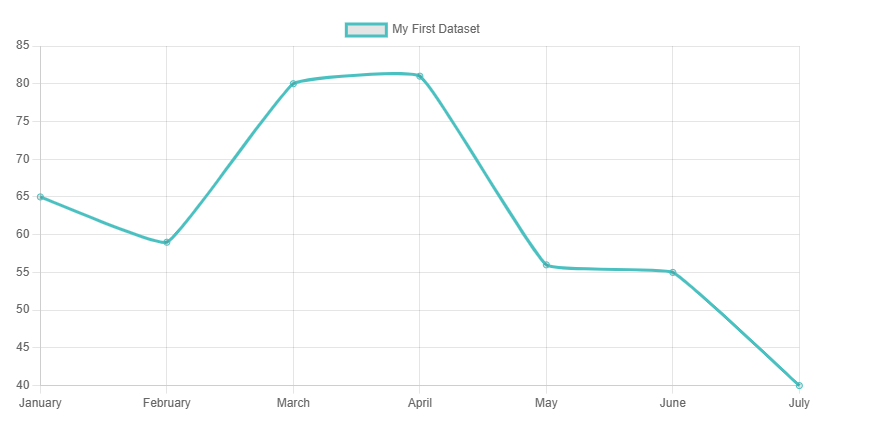
\includegraphics[width=0.8\linewidth]{gambar/Dasar teori/LineChart.png}
	\caption{Bentuk Line Chart}
	\label{gambar1}
\end{figure}

\subsubsection{Bar Chart}
Bar Chart adalah metode untuk menampilkan nilai data dalam bentuk batang vertikal. Grafik ini seringkali digunakan untuk menunjukkan tren data serta membandingkan beberapa set data secara berdampingan [25].

\begin{figure}[H]
	\centering
	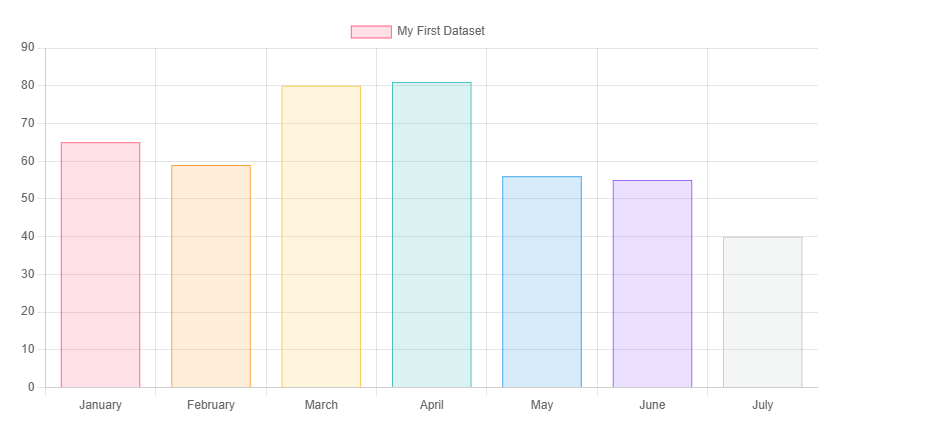
\includegraphics[width=0.8\linewidth]{gambar/Dasar teori/Bar Chart.png}
	\caption{Bentuk Bar Chart}
	\label{gambar1}
\end{figure}

\subsubsection{Scatter Plot}
Scatter plot merupakan salah satu jenis grafik yang membandingkan nilai data numerik dari dua variabel menggunakan titik yang berada dalam koordinat (x,y). Biasanya, jenis grafik ini digunakan untuk membandingkan nilai antar variabel [25]

\begin{figure}[H]
	\centering
	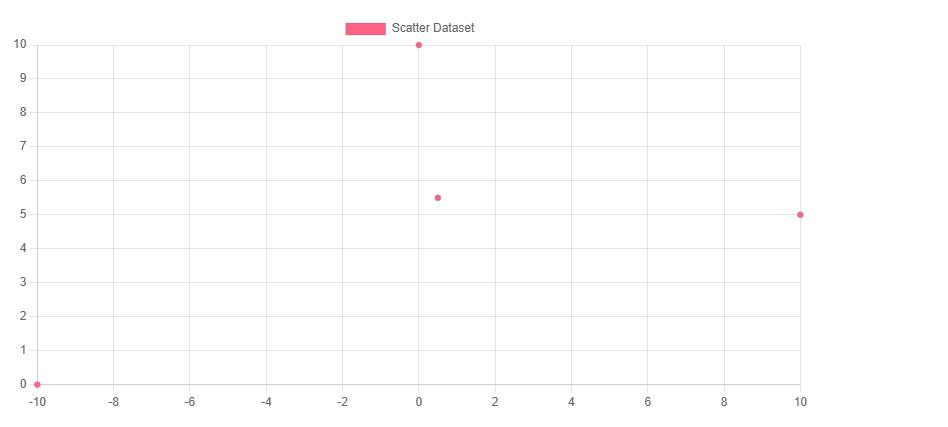
\includegraphics[width=0.8\linewidth]{gambar/Dasar teori/scatter.png}
	\caption{Bentuk Scatter Plot}
	\label{gambar1}
\end{figure}

\subsection{IoT}
Internet of Things (IoT) adalah konsep yang bertujuan untuk memperluas manfaat konektivitas internet yang selalu terhubung. IoT mengacu pada sistem di mana berbagai objek di dunia nyata dapat saling berkomunikasi dalam sebuah jaringan yang terintegrasi dengan internet sebagai perantara utamanya. Secara umum, cara kerja IoT berlandaskan pada tiga elemen utama, yaitu perangkat fisik yang telah dilengkapi modul IoT, perangkat koneksi seperti modem dan router nirkabel untuk menghubungkan ke internet, serta pusat data berbasis cloud yang berfungsi sebagai tempat penyimpanan aplikasi dan basis data. Modul IoT ini akan mengumpulkan serta mengirimkan data dalam rentang waktu tertentu sesuai dengan konfigurasi yang telah ditetapkan [27].

\subsection{Dataset}
Secara umum, dataset didefinisikan sebagai kumpulan data yang dikumpulkan dan disusun dalam suatu format tertentu untuk digunakan dalam analisis lebih lanjut. Definisi dataset didefinisikan sesuai konteks penggunaannya, seperti dalam ilmu komputer, statistik, atau penelitian ilmiah [9]. Pada konteks penelitian ini, dataset ini merupakan data yang dihasilkan secara terus menerus dari perangkat IoT. Format data yang akan digunakan adalah JSON dan akan diuji cobakan sebagai data yang akan ditampilkan dalam visualisasi dan menentukan hasil evaluasi nantinya. 

\subsection{Pengujian Performa}
Performa mengacu pada proses evaluasi, pengukuran, dan penilaian terhadap efisiensi dalam menyelesaikan suatu tugas. Dalam bidang komputasi, performa menggambarkan efektivitas sebuah komputer dalam menjalankan suatu proses. Indikator utama dalam mengukur performa adalah jumlah waktu dan sumber daya yang digunakan untuk menyelesaikan tugas tersebut [28]. Dalam penelitian ini, performa yang diukur antara lain adalah rendering, scalability, dan penggunaan resource CPU dan memori. 

\subsubsection{Rendering}
Rendering merupakan proses pembuatan tampilan visual dalam bentuk gambar atau model 3D. Terdapat 2 jenis metode rendering yang dapat dilakukan, yaitu Hardware rendering dan Software Rendering. Software rendering memanfaatkan CPU untuk memproses dan menampilkan gambar, sementara hardware rendering menggunakan GPU untuk mempercepat proses tersebut [29].

\subsubsection{Scalability}
Konsep ini menggambarkan kemampuan suatu sistem untuk beradaptasi dengan pertambahan elemen atau objek, menangani peningkatan beban kerja secara efisien, serta dapat diperluas sesuai kebutuhan. Dalam proses perancangan sistem, skalabilitas sering menjadi faktor utama yang harus dipenuhi [30].

\subsubsection{CPU}
Berbeda dari implementasi perangkat keras lainnya, CPU merupakan perangkat yang sangat fleksibel karena dapat diprogram melalui perangkat lunak. CPU dianggap sebagai komponen dengan konsumsi energi terbesar dalam sebuah komputer. Oleh karena itu, dalam setiap penelitian, pengukuran penggunaan CPU selalu diperhitungkan untuk memperkirakan energi yang digunakan hanya oleh sebuah program computer. Pengukuran penggunaan CPU dapat ditinjau melalui Task Manager atau dengan skrip yang dibuat melalui terminal [31].

\subsubsection{Footprint Memory}
Footprint memory adalah total jumlah memori yang digunakan oleh suatu program, aplikasi, atau proses pada saat berjalan (runtime). Memory footprint digunakan untuk menggambarkan konsumsi memori dari sebuah aplikasi terhadap sistem komputer. Komponen memory footprint meliputi:
\begin{enumerate}
	\item Private memory yang digunakan hanya pada tab spesifik 
	\item Heap memory yang menyimpan objek dan struktur data dinamis.
	\item Stack memory yang digunakan untuk menyimpan variabel lokal dan kontrol eksekusi fungsi.
	\item Buffer dan cache internal yang menyimpan data sementara dari tab website.
\end{enumerate}

\subsubsection{Scalability}
Konsep ini menggambarkan kemampuan suatu sistem untuk beradaptasi dengan pertambahan elemen atau objek, menangani peningkatan beban kerja secara efisien, serta dapat diperluas sesuai kebutuhan. Dalam proses perancangan sistem, skalabilitas sering menjadi faktor utama yang harus dipenuhi [30].

\subsection{Random Access Memory(RAM)}
Memori adalah komponen dalam komputer yang berfungsi untuk menyimpan program dan data. Memori memiliki berbagai jenis, teknologi, struktur, dan kinerja yang bervariasi, tergantung pada cara informasi disimpan, dibaca, dan ditulis. CPU memiliki tiga tingkat cache, yang juga dikenal sebagai RAM internal. RAM internal membantu meningkatkan kinerja prosesor yang memungkinkan instruksi dikirim ke CPU lebih cepat dibandingkan jika diambil dari RAM eksternal. Saat CPU membutuhkan data, pencarian pertama dilakukan di cache Level 1 (L1), kemudian di Level 2 (L2), dan terakhir di Level 3 (L3). Jika data tidak ditemukan dalam cache, CPU akan mengambilnya dari DRAM [32]. Salah satu bagian dari RAM yang digunakan untuk memproses alokasi memori dinamis adalah heap memory. Heap memory akan menunjukkan distribusi memori di antara objek JavaScript pada halaman dan node DOM terkait. Penggunaan RAM ini dapat dipantau pada komputer, salah satunya melalui Chrome Task Manager pada kolom memory footprint. 

\subsection{Chrome Task Manager}
Task Manager merupakan ekstensi Chrome yang dapat digunakan untuk memantau dan mengelola berbagai proses yang berjalan di dalam browser.  Beberapa hal yang diukur dan ditampilkan oleh Chrome Task Manager antara lain:
\begin{enumerate}
	\item Penggunaan CPU menunjukkan seberapa banyak prosesor yang digunakan oleh setiap proses. 
	\item Memory Footprint mengukur jumlah memori yang digunakan oleh setiap proses, termasuk tab, ekstensi, dan plugin. Hal ini membantu dalam mengidentifikasi proses yang memakan banyak RAM.
	\item Network memantau aktivitas jaringan dari setiap proses sehingga penggunaan bandwith dapat terpantau. 
	\item Process ID merupakan id yang dapat digunakan untuk pelacakan dan diagnostik lebih lanjut.
\end{enumerate}